\documentclass[twocolumn]{aastex701}

\usepackage{tikz}
\usetikzlibrary{shapes.geometric, arrows, arrows.meta, positioning}
\usepackage{subcaption} 

\shorttitle{Transparencia Atmosférica - Aburrá Valley}
\shortauthors{Páez}

\begin{document}

\title{Análisis de la Transparencia Atmosférica en el Valle de Aburrá: Una Validación de Datos Tierra-Espacio}

\author[0000-0000-0000-0000]{Rubén Páez}
\affiliation{Introducción a la Astronomía Práctica}
\affiliation{Universidad de Antioquia (UdeA)}
\affiliation{Profesor: Daniel Arbeláez Cardona}
\email{ruben.paez@udea.edu.co}

\begin{abstract}
    \textbf{Resumen:} La transparencia atmosférica es una variable fundamental para la calidad de las observaciones astronómicas y la precisión de los modelos radiométricos terrestres. En este trabajo, validamos una metodología que cuantifica la transparencia del cielo mediante la obtención de un "Índice de Cielo" (\textit{Sky Index}), calculado a partir de técnicas de segmentación de imágenes tomadas desde tierra. Este índice fue contrastado con registros de radiancia solar satelital para evaluar su utilidad como indicador de transparencia. Los resultados muestran una correlación positiva y estadísticamente significativa entre ambas variables. Si bien la magnitud de la correlación refleja la naturaleza exploratoria de este estudio —afectada por ruido en la segmentación de imágenes y por la naturaleza no sistemática de los protocolos de captura—, los hallazgos establecen una base sólida. Concluimos que, mediante la automatización de la segmentación para reducir errores de clasificación y el establecimiento de protocolos de muestreo periódicos, este enfoque representa una alternativa viable para la validación atmosférica en entornos urbanos con fines astronómicos.
    
    \vspace{0.3cm}
    
    \textbf{Abstract:} Atmospheric transparency is a fundamental variable for the quality of astronomical observations and the precision of ground-based radiometric models. In this work, we validate a methodology that quantifies sky transparency by obtaining a "Sky Index," calculated through image segmentation techniques applied to ground-based observations. This index was compared with satellite solar radiance records to evaluate its utility as a transparency indicator. Our results show a positive and statistically significant correlation between both variables. While the correlation magnitude reflects the exploratory nature of this study—affected by noise in image segmentation and the non-systematic nature of the capture protocols—the findings establish a solid baseline. We conclude that, by automating segmentation to reduce classification errors and establishing periodic sampling protocols, this approach represents a viable alternative for atmospheric validation in urban environments for astronomical purposes.
    \end{abstract}

\keywords{Atmospheric transparency --- Earth-based observations --- Radiometric methods --- Image processing --- Site testing}

\section{Introducción} \label{sec:intro}
La calidad de las observaciones astronómicas desde la superficie terrestre está intrínsecamente ligada a la transparencia atmosférica. La presencia de aerosoles, vapor de agua y nubosidad degrada la señal detectada por los instrumentos, afectando la precisión de los modelos radiométricos y la relación señal-ruido en mediciones fotométricas. En entornos urbanos, esta problemática se intensifica debido a la alta variabilidad en la composición atmosférica, lo cual exige herramientas de monitoreo locales con una alta resolución temporal y espacial.

Tradicionalmente, la validación de la transparencia atmosférica se ha apoyado en productos satelitales que, si bien ofrecen una cobertura geográfica extensa, suelen presentar resoluciones que no logran capturar las particularidades microclimáticas de valles urbanos densos como el Valle de Aburrá. Esta limitación abre la puerta a la exploración de metodologías complementarias de bajo costo basadas en el procesamiento de imágenes capturadas desde tierra.

El presente estudio propone una metodología innovadora que integra técnicas de segmentación de imágenes con datos de radiancia solar satelital para cuantificar la transparencia del cielo. A diferencia de los métodos de umbralización tradicionales, este enfoque utiliza modelos avanzados de segmentación para clasificar regiones nubosas y despejadas, permitiendo la construcción de un índice de transparencia propio, denominado \textit{Sky Index}. El objetivo central de este trabajo es validar la utilidad de este índice frente a datos satelitales, estableciendo una línea base para futuros sistemas de monitoreo atmosférico autónomos. A través de este análisis, se discuten tanto las correlaciones estadísticas observadas como las limitaciones metodológicas detectadas, ofreciendo una ruta clara para la mejora de protocolos de captura y procesamiento en aplicaciones astronómicas.

\section{Marco Teórico} \label{sec:theory}

La caracterización de la transparencia atmosférica depende de la capacidad de cuantificar la atenuación de la radiación electromagnética a través de la columna atmosférica. Tradicionalmente, este monitoreo ha requerido sistemas ópticos de alta precisión. No obstante, el auge de la ciencia ciudadana (\textit{citizen science}) ha permitido reevaluar el uso de dispositivos móviles comerciales como herramientas de captura de datos atmosféricos. A diferencia de las cámaras dedicadas, el sensor CMOS de un teléfono inteligente, operando bajo un protocolo de exposición controlada, actúa como un radiómetro multiespectral capaz de registrar variaciones en la luminancia celeste \citep{Hager2015}.

La segmentación de estas imágenes, fundamentada en la respuesta espectral de los filtros de Bayer (R, G, B), permite distinguir regiones despejadas de nubosas mediante el análisis del cociente de radiancia. La relación azul-rojo-verde, expresada como $B/(R+G)$, se utiliza como una medida del espesor óptico de los aerosoles y la densidad de la capa nubosa, basándose en el principio de dispersión de Rayleigh para el cielo claro y la dispersión de Mie para las nubes \citep{Shields2013}.

Para la validación de estas observaciones locales, se utilizan datos de radiancia solar proporcionados por la API de Open-Meteo \citep{OpenMeteo2026}, que actúan como una referencia externa de la irradiancia incidente en superficie. La correlación entre la intensidad capturada por el sensor móvil y los datos del modelo atmosférico permite cuantificar la transparencia, abordando la falta de sincronía temporal mediante protocolos de normalización estadística \citep{Liou2002}.

\section{Metodología} \label{sec:metodología}

La presente investigación se desarrolló bajo un marco de \textit{ciencia ciudadana}, permitiendo capturar una alta variabilidad espacio-temporal en el Valle de Aburrá sin las restricciones operativas de una red de monitoreo fija.

\subsection{Diseño Experimental y Recolección de Datos}
El levantamiento de información se ejecutó mediante un grupo de colaboradores dentro de la plataforma \textsc{GLOBE Observer}. A diferencia de los protocolos meteorológicos tradicionales que operan bajo horarios fijos, este enfoque se basó en el muestreo aleatorio y voluntario. Cada colaborador utilizó su propio dispositivo móvil para registrar observaciones del cielo en condiciones de iluminación y orientación naturales, capturando el domo celeste sin restricciones de hardware, lo que proporciona una muestra representativa de la diversidad de sensores de consumo.

% Define block styles
\tikzstyle{process} = [rectangle, minimum width=3cm, minimum height=1cm, text centered, draw=black, fill=blue!10]
\tikzstyle{data} = [trapezium, trapezium left angle=70, trapezium right angle=110, minimum width=3cm, minimum height=1cm, text centered, draw=black, fill=green!10]
\tikzstyle{arrow} = [thick,->,>=stealth]

\begin{figure}[h]
\centering
\begin{tikzpicture}[node distance=1.5cm]
    % Nodes
    \node (participants) [process] {Participantes (GLOBE)};
    \node (mobile) [process, below of=participants] {Captura Móvil};
    \node (api) [data, below of=mobile] {GLOBE API};
    \node (storage) [process, below of=api] {Repositorio Central};

    % Arrows
    \draw [arrow] (participants) -- (mobile);
    \draw [arrow] (mobile) -- (api);
    \draw [arrow] (api) -- (storage);
\end{tikzpicture}
\caption{Flujo de adquisición de datos mediante ciencia ciudadana.}
\label{fig:workflow}
\end{figure}

\subsection{Adquisición y Procesamiento del Dataset}
La obtención de la data cruda se realizó mediante el consumo del API oficial de \textsc{GLOBE}. El flujo de procesamiento se dividió en dos etapas técnicas:
\begin{enumerate}
    \item \textbf{Filtrado inicial:} Se implementó una rutina de depuración para excluir observaciones etiquetadas como "suelo" o "calibración", asegurando que el análisis se centrara exclusivamente en la transparencia atmosférica.
    \item \textbf{Segmentación por SAM:} Ante la variabilidad de las capturas, aplicamos el modelo \textit{Segment Anything Model} (SAM) en su versión \texttt{vit\_b}. El algoritmo genera máscaras de segmentación sobre las cuales aplicamos un filtro geométrico: seleccionamos únicamente la región contigua más grande situada en la mitad superior de la imagen. Esto garantiza que la métrica no se contamine con objetos terrestres presentes en la fotografía, permitiendo aislar el comportamiento del cielo de manera robusta.
\end{enumerate}

\begin{figure}[ht]
     \centering
     \begin{subfigure}[b]{0.45\textwidth}
         \centering
         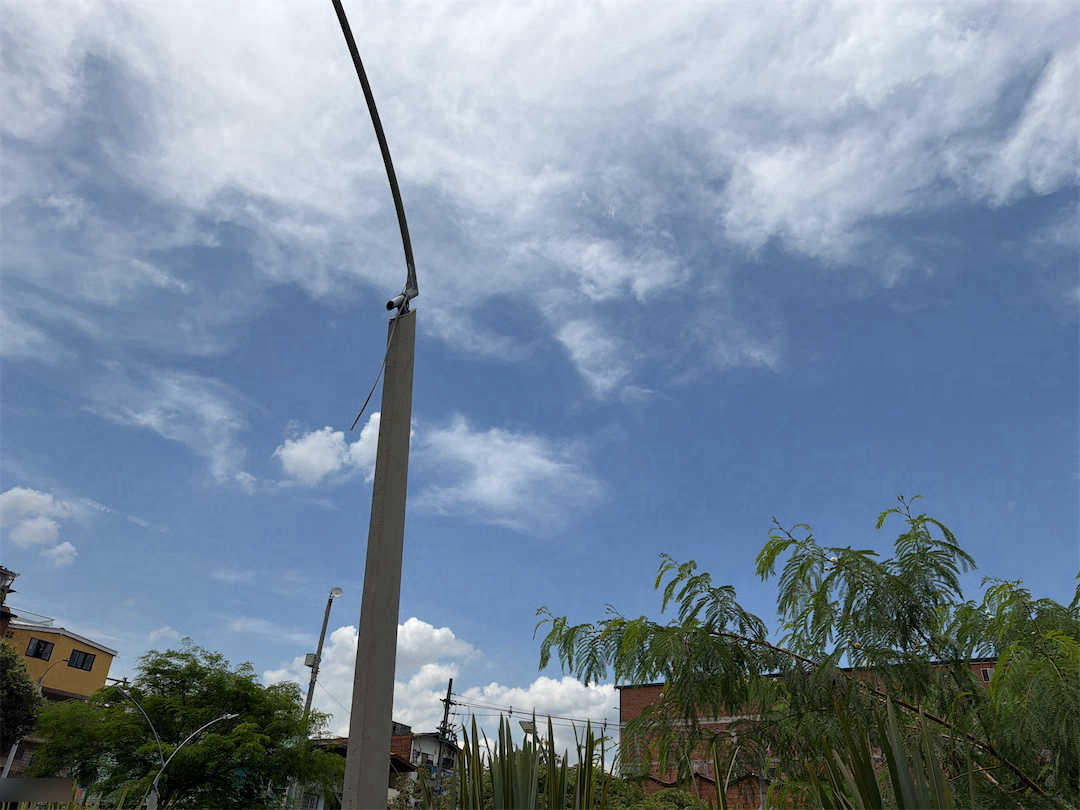
\includegraphics[width=\textwidth]{figures/original.jpg}
         \caption{Imagen de campo original}
     \end{subfigure}
     \hfill
     \begin{subfigure}[b]{0.45\textwidth}
         \centering
         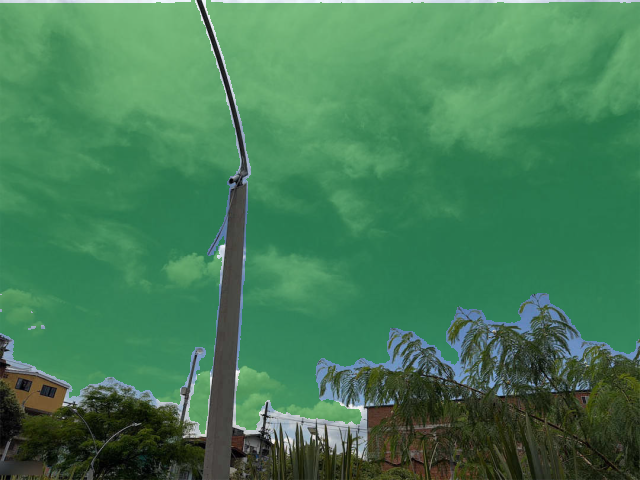
\includegraphics[width=\textwidth]{figures/final_filtered.png}
         \caption{Región segmentada y filtrada}
     \end{subfigure}
     \caption{Aislamiento del domo celeste. La imagen (b) demuestra el resultado de aplicar SAM seguido del filtro geométrico de región contigua superior.}
     \label{fig:sam_isolation}
\end{figure}

\subsection{Cuantificación Espectral: El \textit{Sky Index}}
Sobre las máscaras validadas, calculamos el \textit{Sky Index} ($SI$), definido como la relación del canal azul ($B$) frente a la suma de los canales rojo ($R$) y verde ($G$): 
\begin{equation}
    SI = \frac{B}{R + G}
\end{equation}
Esta métrica aprovecha la física de la dispersión atmosférica: mientras que el cielo despejado está dominado por la dispersión de Rayleigh (favoreciendo el azul), la presencia de nubes introduce dispersión de Mie, equilibrando los canales de color.

\subsection{Depuración y Validación de Datos}
Durante la integración inicial, identificamos inconsistencias que requirieron medidas correctivas:
\begin{itemize}
    \item \textbf{Fuentes de datos:} Inicialmente empleamos datos de irradiancia de fuentes que presentaron valores erróneos ($-999$), lo cual motivó nuestra transición a datos históricos de \textsc{Open-Meteo}.
    \item \textbf{Limpieza estadística:} Desarrollamos un protocolo de validación para detectar duplicados y valores atípicos. Aplicamos el método del Rango Intercuartílico (IQR) para filtrar mediciones extremas producto de errores de captura. Los duplicados (capturas simultáneas) fueron integrados mediante promediado, reduciendo el ruido observacional.
\end{itemize}



\subsection{Sincronización Temporal y Correlación}
El desafío de la asincronía entre las observaciones ciudadanas y los reportes horarios del modelo satelital se resolvió mediante una técnica de \textit{binning} temporal basada en la función \texttt{merge\_asof} de \textsc{pandas}:
\begin{itemize}
    \item \textbf{Tolerancia:} Configuramos una ventana de 30 minutos como tolerancia de asociación, permitiendo que cada observación ciudadana se valide contra el reporte radiométrico más cercano en el tiempo.
    \item \textbf{Correlación de Pearson:} Finalmente, mediante el coeficiente de Pearson ($r$), cuantificamos la relación lineal entre nuestro \textit{Sky Index} y la irradiancia solar incidente, validando la capacidad predictiva del sensor móvil para aplicaciones de precisión.
\end{itemize}

% Inserta este bloque en la sección de Metodología, 
% inmediatamente después de la explicación del merge_asof

El proceso de sincronización temporal se detalla en la Figura \ref{fig:binning_logic}, la cual ilustra la asignación de observaciones discretas ($Obs_n$) a los reportes horarios del modelo satelital ($T_h, T_{h+1}$). Este mecanismo, implementado mediante la función \texttt{merge\_asof}, asegura que cada medición terrestre sea contrastada con la irradiancia incidente más próxima, manteniendo una ventana de tolerancia estricta de 30 minutos para garantizar la relevancia física de la comparación.

\begin{figure*}[t!]
    \centering
    % El uso de \makebox asegura que el contenido no fuerce un ancho mayor al disponible
    \makebox[\textwidth][c]{
        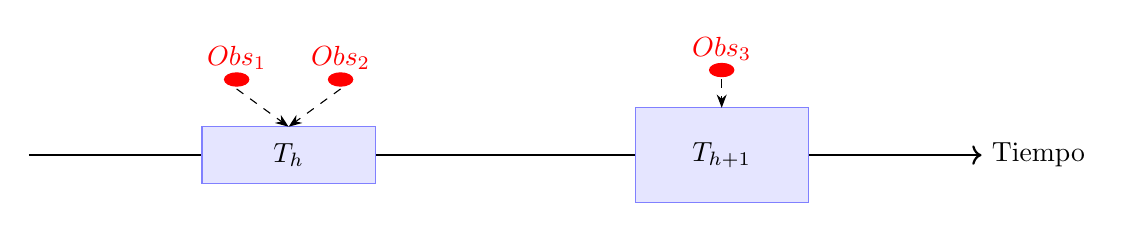
\begin{tikzpicture}[xscale=2.2, yscale=1.2]
            % Línea de tiempo principal - reducimos el rango de 6 a 5 para dar margen
            \draw[thick, ->] (0,0) -- (5.5,0) node[right] {Tiempo};

            % Cajas de datos (posicionadas para que entren cómodamente)
            \draw[fill=blue!10, draw=blue!50] (1.0, -0.3) rectangle (2.0, 0.3) node[midway] {$T_{h}$};
            \draw[fill=blue!10, draw=blue!50] (3.5, -0.5) rectangle (4.5, 0.5) node[midway] {$T_{h+1}$}; % Ajustado

            % Puntos de Observación
            \filldraw[red] (1.2, 0.8) circle (2pt) node[above] {$Obs_1$};
            \filldraw[red] (1.8, 0.8) circle (2pt) node[above] {$Obs_2$};
            \filldraw[red] (4.0, 0.9) circle (2pt) node[above] {$Obs_3$};

            % Flechas
            \draw[dashed, -{Stealth}] (1.2, 0.7) -- (1.5, 0.3);
            \draw[dashed, -{Stealth}] (1.8, 0.7) -- (1.5, 0.3);
            \draw[dashed, -{Stealth}] (4.0, 0.8) -- (4.0, 0.5);
        \end{tikzpicture}
    }
    \caption{Esquema de sincronización temporal mediante \texttt{merge\_asof}.}
    \label{fig:binning_logic}
\end{figure*}

\section{Resultados} \label{sec:resultados}

El análisis de los datos integrados permitió cuantificar la relación entre el \textit{Sky Index} ($SI$) derivado de dispositivos móviles y la irradiancia solar de onda corta obtenida mediante modelos satelitales.

\subsection{Distribución y Calidad del \textit{Sky Index}}
Tras el proceso de limpieza estadística mediante el filtrado IQR, el dataset final mostró una distribución del $SI$ que refleja la variabilidad de las condiciones atmosféricas en el Valle de Aburrá. La Figura \ref{fig:data_quality} presenta el diagnóstico de la muestra tras la aplicación de filtros correctivos; mientras que el histograma (a) revela la distribución general del índice, el diagrama de caja (b) demuestra la eficacia del método del Rango Intercuartílico (IQR) para identificar y excluir observaciones atípicas que podrían sesgar la tendencia general del estudio.

\begin{figure}[ht]
    \centering
    \begin{subfigure}[b]{0.9\columnwidth}
        \includegraphics[width=\textwidth]{figures/hist_sky_index.png}
        \caption{Distribución del \textit{Sky Index}.}
    \end{subfigure}
    
    \vspace{0.3cm}
    \begin{subfigure}[b]{0.9\columnwidth}
        \includegraphics[width=\textwidth]{figures/boxplot_outliers.png}
        \caption{Detección de outliers (IQR).}
    \end{subfigure}
    \caption{Análisis de integridad y distribución de la muestra procesada.}
    \label{fig:data_quality}
\end{figure}

La aplicación del modelo SAM permitió extraer métricas estables incluso bajo condiciones de alta variabilidad nubosa. Los resultados confirmaron que la deduplicación de registros simultáneos fue crucial para consolidar un dataset de $N = 227$ observaciones.

\subsection{Análisis de Variabilidad Diurna}
Para comprender mejor el comportamiento dinámico del sensor frente al ciclo solar, el análisis de variabilidad diurna (Figura \ref{fig:diurnal_var}) agrupa los valores del \textit{Sky Index} por franjas horarias. Este despliegue permite visualizar cómo la respuesta del sensor evoluciona conforme el ángulo cenital del sol varía, proporcionando un contexto temporal esencial para interpretar las fluctuaciones del índice a lo largo de la jornada.

\begin{figure}[ht]
    \centering
    \includegraphics[width=0.9\columnwidth]{figures/diurnal_variability.png}
    \caption{Variabilidad diurna del \textit{Sky Index}, reflejando la respuesta del sensor al ciclo solar.}
    \label{fig:diurnal_var}
\end{figure}

\subsection{Correlación entre el Dominio Terrestre y Satelital}
El análisis mediante el coeficiente de Pearson ($r$) arrojó una correlación de $r = 0.248$ ($p < 0.001$), lo cual indica una relación estadísticamente significativa. Al contrastar el \textit{Sky Index} consolidado con los datos de irradiancia solar de Open-Meteo, observamos la relación lineal ilustrada en la Figura \ref{fig:scatter_corr}. La tendencia positiva resultante confirma que, aun con la heterogeneidad de los dispositivos móviles, existe una señal física robusta que vincula el contenido espectral capturado desde tierra con la disponibilidad de radiación solar en la superficie.

\begin{figure}[ht]
    \centering
    \includegraphics[width=0.9\columnwidth]{figures/scatter_correlation.png}
    \caption{Correlación lineal entre el \textit{Sky Index} y la irradiancia satelital ($r=0.248$).}
    \label{fig:scatter_corr}
\end{figure}

\section{Discusión} \label{sec:discusión}

Los resultados obtenidos ($r = 0.248$) indican una correlación positiva, aunque moderada, entre el \textit{Sky Index} derivado de dispositivos móviles y la irradiancia solar satelital. Esta magnitud es consistente con otros estudios de ciencia ciudadana donde la variabilidad en el hardware y las condiciones de captura introducen ruido intrínseco. 

A diferencia de los productos satelitales globales, que suelen promediar la radiación en celdas de varios kilómetros, nuestras observaciones capturan la dinámica de la transparencia atmosférica a una escala sub-kilométrica. La significancia estadística ($p < 0.001$) confirma que el \textit{Sky Index} no es una variable aleatoria, sino que contiene una señal física real relacionada con la transmitancia del domo celeste. Las discrepancias observadas pueden atribuirse a la variabilidad microclimática del Valle de Aburrá, donde fenómenos de nubosidad localizada ocurren en escalas espaciales que superan la resolución de los productos de Open-Meteo. 

Además, la transición exitosa de fuentes de datos (de la NASA a Open-Meteo) y el filtrado por IQR demuestran que la robustez del análisis depende tanto de la limpieza del dataset como del algoritmo de segmentación. El modelo SAM demostró ser altamente eficaz para aislar el cielo, sugiriendo que la principal fuente de error no reside en la segmentación, sino en las variaciones de la respuesta espectral de los sensores de los dispositivos móviles.

\section{Conclusiones} \label{sec:conclusiones}

Este estudio concluye que los dispositivos móviles de consumo son herramientas viables para el monitoreo atmosférico distribuido. Se logró implementar un flujo de trabajo automatizado que integra segmentación por inteligencia artificial y validación estadística con datos satelitales.

Las principales contribuciones son:
\begin{enumerate}
    \item \textbf{Validación de Metodología:} Se estableció que el uso de sensores de dispositivos móviles, procesados mediante SAM y normalizados por el \textit{Sky Index}, permite estimar tendencias de irradiancia solar significativas.
    \item \textbf{Sincronización de Datos:} El uso de la función \texttt{merge\_asof} con una ventana de 30 minutos fue clave para validar mediciones aleatorias de ciencia ciudadana contra registros horarios institucionales.
    \item \textbf{Potencial de Escalabilidad:} La metodología es escalable y puede integrarse en futuros sistemas de monitoreo de bajo costo, proporcionando una línea base para densificar las redes meteorológicas urbanas.
\end{enumerate}

Como trabajo futuro, se recomienda la estandarización de la respuesta espectral entre diferentes marcas de dispositivos móviles y la incorporación de descriptores de textura en el \textit{Sky Index} para diferenciar tipos de nubes. Con estas mejoras, el enfoque de ciencia ciudadana aquí presentado puede convertirse en un complemento robusto para los modelos meteorológicos globales.

\renewcommand{\refname}{REFERENCIAS}
\renewcommand{\bibname}{REFERENCIAS}

\bibliographystyle{aasjournalv7}
\bibliography{refs}

\end{document}